\section{Problem Description}\label{sec:problem}

%==============================
\subsection{Workspace and Robots}\label{subsec:ws}
The workspace is a bounded planar region
$\mathcal{W}\subset\mathbb{R}^2$ that contains two types of
obstacles. A set $\mathcal{O}$ represents immovable structures,
while a set of $M$ movable rigid polygons is defined as
$\boldsymbol{\Omega}\triangleq\{\Omega_1,\cdots,\Omega_M\}\subset\mathcal{W}$.
Each movable obstacle $\Omega_m$ is characterized by its mass
$\mathsf{M}_m$, inertia $\mathsf{I}_m$, frictional parameters
(either identified or estimated), and state
$\mathbf{s}_m(t)\triangleq(\mathbf{x}_m(t),\psi_m(t))$,
where $\mathbf{x}_m(t)\in\mathbb{R}^2$ is the planar position of its centroid
and $\psi_m(t)\in\mathbb{R}$ its orientation angle. The region occupied by
$\Omega_m$ at time $t$ is denoted $\Omega_m(t)$.
Moreover, a small team of $N$ robots, indexed as
$\mathcal{R}\triangleq\{R_1,\cdots,R_N\}$, operates as a cooperative unit.
Each robot $R_i$ is modeled as a rigid body with state
$\mathbf{s}_{R_i}(t)\triangleq(\mathbf{x}_{R_i}(t),\psi_{R_i}(t))$,
where $\mathbf{x}_{R_i}(t)\in\mathbb{R}^2$ is its position and
$\psi_{R_i}(t)\in\mathbb{R}$ its orientation. The footprint of $R_i$ is
denoted $R_i(t)$. The instantaneous free space is given by:
\begin{equation}\label{eq:freespace}
\widehat{\mathcal{W}}(t)\triangleq\mathcal{W}\setminus\Big(
\mathcal{O}\cup\{\Omega_m(t)\}_{m=1}^{M}\cup\{R_i(t)\}_{i=1}^{N}
\Big),
\end{equation}
where $\widehat{\mathcal{W}}(t)$ excludes regions occupied by immovable
obstacles, movable obstacles, and robots.

%==============================
\subsection{External Vehicle and Clearance Goal}\label{subsec:vehicle}
An external vehicle $\texttt{V}$ of radius $W/2>0$ must navigate within the workspace
from a start configuration $\mathbf{s}_\texttt{V}^{\texttt{S}}$ to a goal configuration
$\mathbf{s}_\texttt{V}^{\texttt{G}}$. Since movable obstacles may obstruct the way, a
direct passage is not always feasible. Feasibility at time $t$ is captured by
the $W$-clearance condition
\begin{equation}\label{eq:wclear}
\exists\,\mathcal{P}^W_\texttt{V}\subset\widehat{\mathcal{W}}(t):\
\mathbf{s}_\texttt{V}^{\texttt{S}}\leadsto\mathbf{s}_\texttt{V}^{\texttt{G}},\;
\texttt{clr}(\mathcal{P}^W_\texttt{V})\ge W,
\end{equation}
where $\mathcal{P}^W_\texttt{V}$ is a continuous curve connecting start and goal inside
the free space, and $\texttt{clr}(\mathcal{P}^W_\texttt{V})$ denotes its minimum clearance
to surrounding obstacles.

%==============================
\subsection{Collaborative Pushing Modes}\label{ss:interaction_mode}
Thus, the robots may actively reconfigure $\boldsymbol{\Omega}$ by pushing obstacles.
The interaction with obstacle $\Omega_m$ is described by a pushing mode
$\boldsymbol{\xi}_m\triangleq(\mathcal{C}_m,\mathbf{u}_m)$,
where $\mathcal{C}_m\in(\partial\Omega_m)^N$ is the set of contact points
established by the robots, and $\mathbf{u}_m\in\mathbb{R}^{2N}$ encodes the body-frame forces
or an equivalent wrench profile. The admissible set of
modes is $\Xi_m$, determined by contact geometry and frictional limits.
Furthermore, the system evolution under a pushing mode
is captured by the transition operator below:
\begin{equation}\label{eq:transition}
  \mathbf{S}(t^+)\triangleq\Phi\big(\mathbf{S}(t),\,m,\,\boldsymbol{\xi}_m\big),
\end{equation}
where $\mathbf{S}(t)$ stacks all robot and obstacle states. The operator
$\Phi$ models the joint dynamics of robots and obstacles under contact. In
general, $\Phi$ is not available in closed form and is instead evaluated
through physics simulation.

%==============================================
\begin{figure*}[t!]
  \centering
  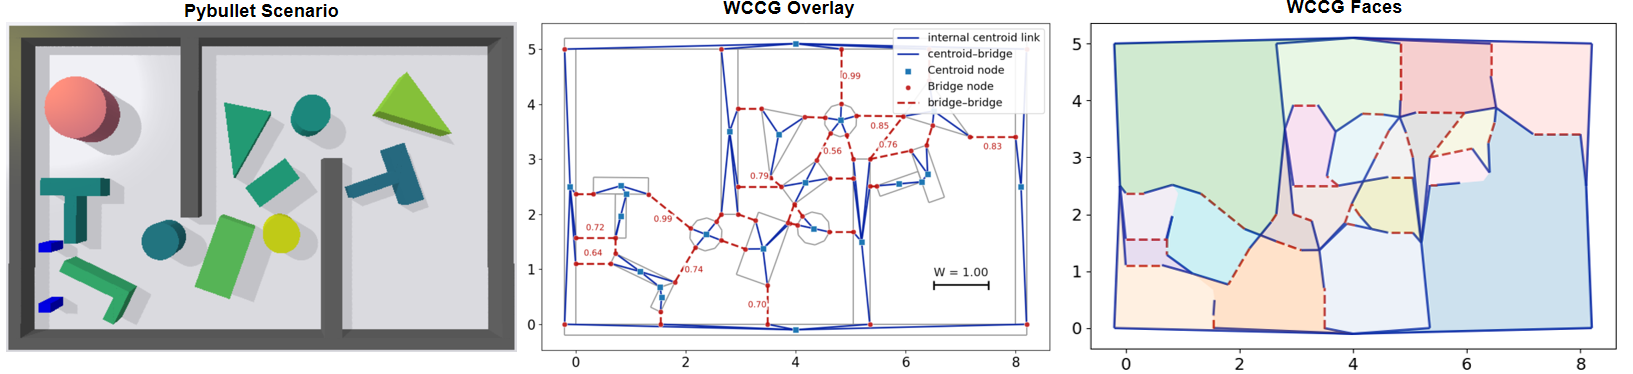
\includegraphics[width=\linewidth]{figures/wccg.pdf}
  \vspace{-0.2in}
  \caption{Illustration of the W--Clearance Connectivity Graph (WCCG).
\textbf{Left:} Cluttered PyBullet scenario with the immovable walls and movable objects;
\textbf{Middle:} WCCG overlay with the centroid nodes (blue squares), bridge nodes
(red circles), centroid--bridge edges (blue), and bridge--bridge edges (red dashed)
annotated by the gap widths;
\textbf{Right:} Induced faces of the WCCG, where the colors indicate distinct connected
regions.}
  \label{fig:wccg}
  \vspace{-0.2in}
\end{figure*}
%==============================================

%==============================
\subsection{Problem Statement}\label{subsec:objective}
The goal is to compute a hybrid schedule for the robots that reconfigures the movable
obstacles so that the vehicle admits a $W$-feasible path from start to goal.
The overall schedule for the robotic fleet is defined as:
\begin{equation}\label{eq:schedule}
\pi\triangleq\big\{(m_k,\boldsymbol{\xi}_k,\Delta t_k)\big\}_{k=1}^{K},
\end{equation}
where $\Omega_{m_k}\in \boldsymbol{\Omega}$ specifies the movable obstacle to manipulate,
$\boldsymbol{\xi}_k\in\Xi_{m_k}$ is the pushing mode, and
$\Delta t_k>0$ the duration of execution.
Thus, the optimization problem balances the execution time and the physical effort
of the clearance process, subject to various constraints, i.e.,
\begin{equation}\label{eq:problem}
\underset{\pi}{\textbf{min}}\ \Big{\{} T+\alpha\sum_{k=1}^{K}
J\!\left(m_k,\,\boldsymbol{\xi}_k,\,\mathbf{S}(\tau_k)\right)\Big{\}},
\end{equation}
where $T\triangleq\sum_{k=1}^{K}\Delta t_k$ is the total task duration,
$\alpha>0$ is a trade-off parameter, and $J(\cdot)$ is a simulation-based
control effort or feasibility cost evaluated at state $\mathbf{S}(\tau_k)$.
Note that the above optimization
problem is constrained by \eqref{eq:freespace}, \eqref{eq:wclear}, and
\eqref{eq:transition}, which jointly ensure collision-free evolution within
the workspace, valid dynamic transitions under pushing, and a terminal
$W$-clearance path for the vehicle.

% ==============================
\begin{remark}\label{remark:uniqueness}
  Problem~\eqref{eq:problem} above uniquely couples obstacle selection, pushing
  modes, and timing into a single hybrid optimization. This yields a
  combinatorial search space far more complex than classical NAMO, where
  prior work often assumes simple object shapes or hand-crafted contact
  modes~\cite{wang2006multi,goyal1989limit,chen2015occlusion,tang2023combinatorial}.
  \hfill $\blacksquare$
\end{remark}
% ==============================
